
%% Article Template
 \documentclass{scrartcl}
 
 %% UTF8 Encoding
 \usepackage[utf8]{inputenc}
 \usepackage[nenglish]{}
 \usepackage[T1]{fontenc}
 \usepackage{lmodern}
 \usepackage{subcaption}
 \usepackage{setspace}
\usepackage{booktabs} % For formal tables`
\usepackage{graphicx}
 
\title{Preliminary Results}
\author{Cédric Milinaire}
\date{Summer period 2019}
\begin{document}

\begin{titlepage}
\maketitle
\end{titlepage} 
 \begin{abstract}
     This document is used to summarize current results. 
 \end{abstract}
\listoffigures
\listoftables
\newpage
 \begin{abstract}
     This document is used to summarize current results. 
 \end{abstract}
\section{Sampling}
For Table \ref{tab:sampling_stats} the text8 dataset was used, all words that occured less than 5 times were deleted from the dataset before each sampling technique.

\begin{table*}[h]\centering
    \caption{Statistics about dataset with different sampling techniques}
    %\scriptsize
    \begin{tabular}{l r r r r}%
        \toprule
      &    \textbf{w/o sampling} & \textbf{Online Sampling} & \textbf{Mikolov} & \textbf{w/o outliers}  \\%
        \midrule%
        Min     &   34 & 34 & 34 & 7 \\%
       Max    & 9 Mio. & 0.36 Mio. & 0.36 Mio & 590 \\%
      	QTR1      & 79 & 79 & 79&30\\%
         Median &166 & 166 & 166 & 54 \\%
       QTR3     & 533 & 533 & 534 & 123\\%
       QTR3 + 1.5IQR   & 1214 & 1214 & 1217 &227  \\%
               \bottomrule%
       Mean & 2227 & 1125 & 1125 & 100\\%
   \end{tabular}%
   \label{tab:stats_pairs}%
\end{table*}
\begin{table*}[h]\centering
    \caption{Statistics about dataset with different sampling techniques}
    %\scriptsize
    \begin{tabular}{l r r r r}%
        \toprule
      &    \textbf{w/o sampling} & \textbf{Online Sampling} & \textbf{Mikolov} & \textbf{w/o outliers}  \\%
        \midrule%
        Size of Ds   (in words)     &  17 Mio.& 17 Mio. & 8 Mio.& 2.8 Mio.\\%
        Number of Pairs       & 141 Mio. & 71 Mio. & 71. Mio & 6 Mio. \\%
        Number of Sentences         & 0.8 Mio & 0.8 Mio & 0.4 Mio  & 0.1 Mio.\\%
        Vocabulary Size & 0.25 Mio & 0.25 Mio & 0.25 Mio & 0.06 Mio. \\%
        \bottomrule%
   \end{tabular}%
   \label{tab:sampling_stats}%
\end{table*}
\newpage


\begin{figure}
\centering
\begin{minipage}{.3\textwidth}
  \centering
  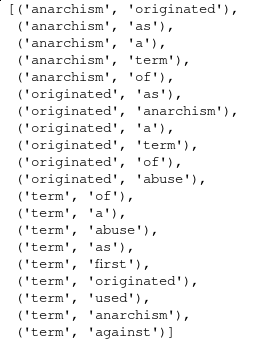
\includegraphics[scale=0.69]{online_sampling_example}
  \captionof{figure}{Online Sampling}
  \label{fig:test1}
\end{minipage}%
\begin{minipage}{.3\textwidth}
  \centering
  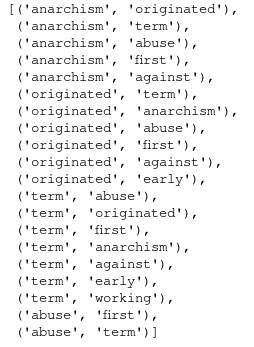
\includegraphics[scale=0.69]{preprocessing_sampling_example}
  \captionof{figure}{Preprocessing S.}
  \label{fig:test2}
\end{minipage}
\begin{minipage}{.3\textwidth}
  \centering
  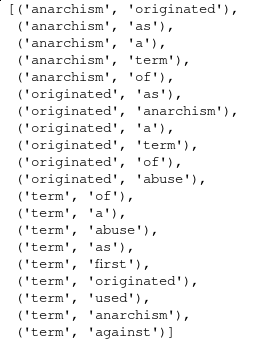
\includegraphics[scale=0.69]{online_sampling_example}
  \captionof{figure}{No Sampling}
  \label{fig:test2}
\end{minipage}
\end{figure}


\section{ Boxplots}
\begin{figure}[h!]
\caption{Distribution of the number of pairs per context word without sampling}
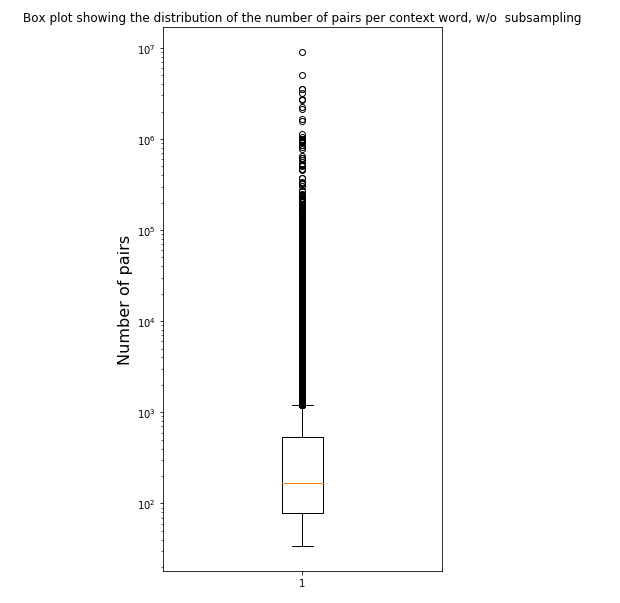
\includegraphics[scale=0.4]{no_sampling_boxplot}
\centering
\end{figure}

\begin{figure}[h!]
\caption{Distribution of the number of pairs per context word with online sampling}
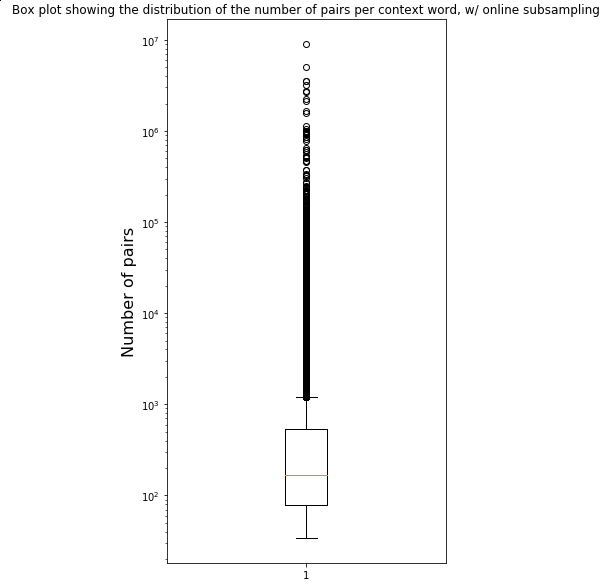
\includegraphics[scale=0.4]{online_sampling_boxplot}
\centering
\end{figure}

\begin{figure}[h!]
\caption{Distribution of the number of pairs per context word with preprocessing sampling}
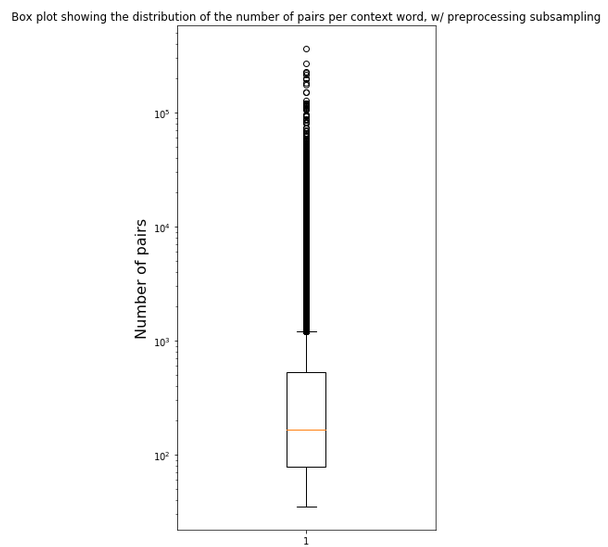
\includegraphics[scale=0.45]{preprocessing_sampling_boxplot}
\centering
\end{figure}

\newpage
\section{Batch\_size}
This section shows a plot of the batch size per batch.
\begin{figure}[h!]
\caption{Batch size per batch}
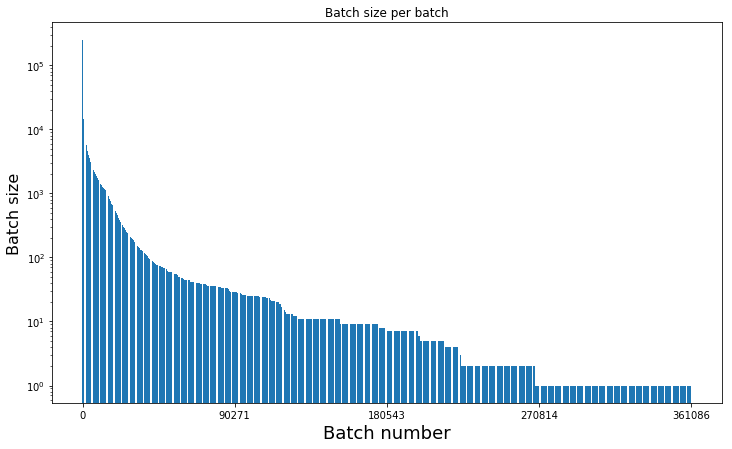
\includegraphics[scale=0.65]{batch_sizes}
\centering
\end{figure}
\section{Results}
Figure \ref{fig:results_w/o_outliers} shows the results of the training of the text8 dataset without outliers. Those results are to be taken very lightly for two reasons: 
\begin{enumerate}
\item The data set is very small, i.e 60k vocabulary
\item To assess word similarity only 12 words from the data set were taken. As those were the only one that are in the data set without outliers and in the wordsim dataset. 
\end{enumerate}

Figure shows that the deletion of the specific word ``the`` does not hinder performance. 

\begin{figure}[h!]
\caption{Results text8 without the word ``the``}
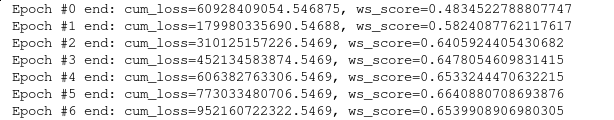
\includegraphics[scale=0.65]{results_without_the}
   \label{fig:results_w/o_outliers}%

\centering
\end{figure}

\begin{figure}[h!]
\caption{Results text8 without outliers}
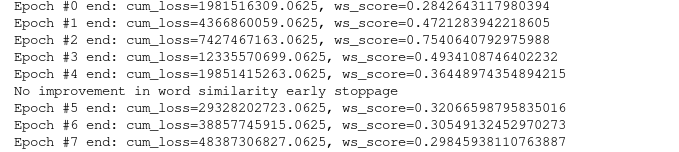
\includegraphics[scale=0.65]{text8_without_outliers}
   \label{fig:results_w/o_outliers}%

\centering
\end{figure}


\end{document}

